\section{Entity relationship diagram}
\subsection{Description}

\begin{flushleft}
Afin de sauvegarder, modifier et supprimer des données, il est nécessaire d'implémenter la notion de factures dans la base de données. C'est pourquoi, ce diagramme illustre l'ajout de factures.
\end{flushleft}

\begin{flushleft}
Tout d'abord, une facture est liée à un contrat. C'est pourquoi, nous retrouvons une liaison entre un contrat et une facture. En outre, un élément \emph{id-factures} a été ajouté à l'entité \emph{contrat} afin de relier les 2.\footnote{\emph{id-factures} étant une Primary Key}
\end{flushleft}

\begin{flushleft}
Ensuite, l'entité \textbf{factures} regroupe plusieurs variables : 
\end{flushleft}
\begin{enumerate}[-]

\item \emph{id-contrat} relie la facture au contrat avec un varchar de 10 caractères.

\item \emph{statut} contient une valeur binaire du statut de paiement.

\item \emph{ideal-accompte} contient une valeur double de l'acompte proposé par l'application.

\item \emph{methode-paiement} contient une valeur binaire du mode de paiement.

\item \emph{paiement-informations} contient un varchar avec les informations bancaires du client.

\end{enumerate}

\newpage
\begin{figure}[h]
\subsection{Schéma}
\centering
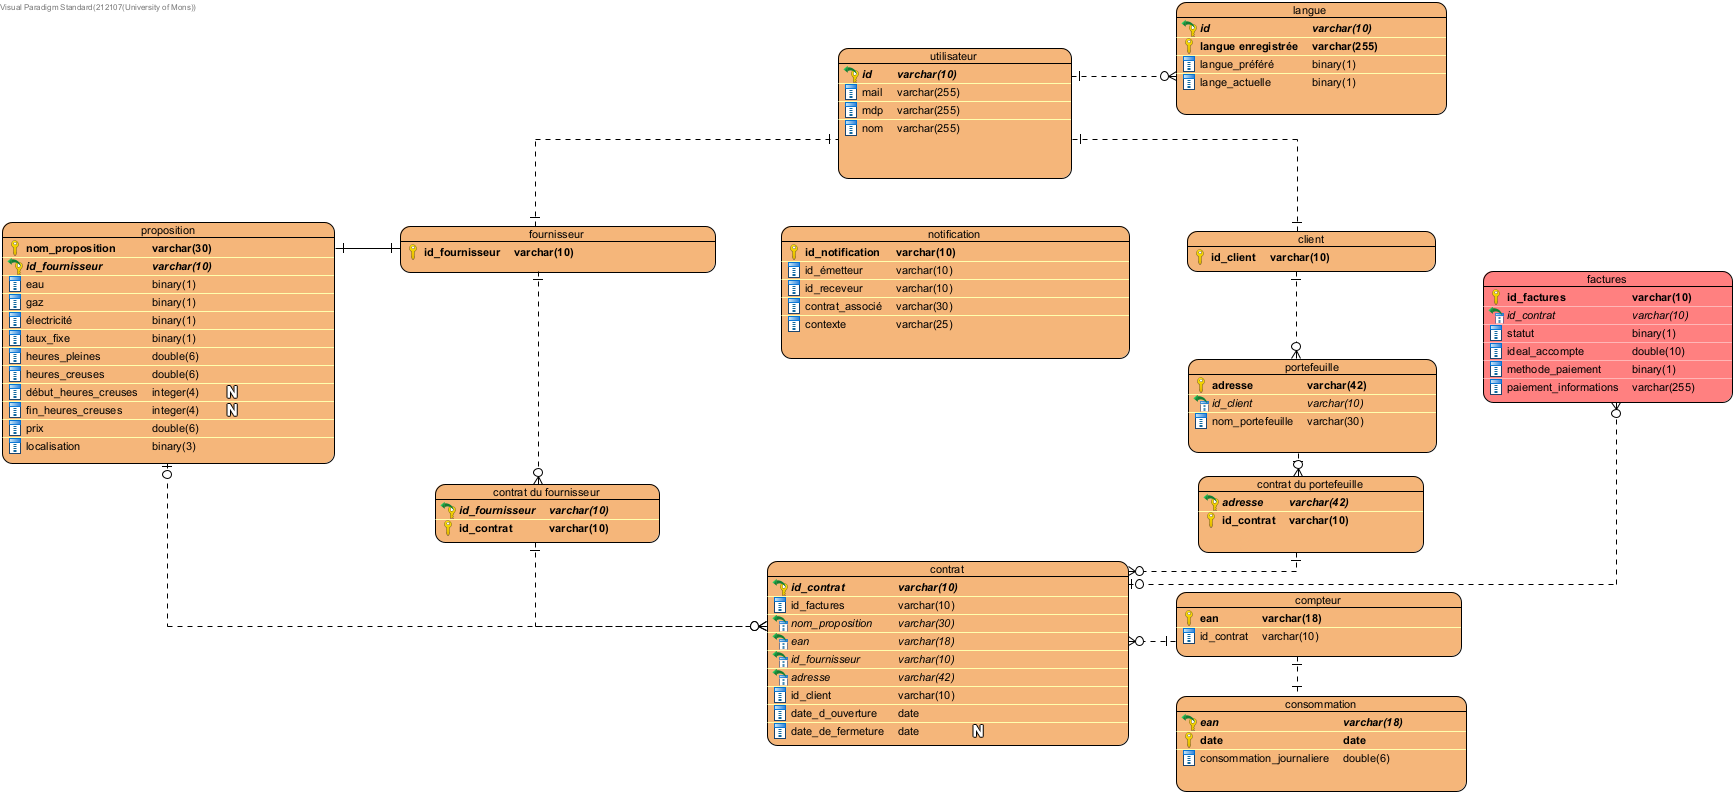
\includegraphics[width = 1.2\textwidth]{extension-maxime/bdd/img/bdd-extension.png}
\end{figure}
